\documentclass[tikz,border=3mm]{standalone}
% Shared TikZ defaults
\usepackage{tikz}
\usetikzlibrary{arrows.meta,positioning,shapes.geometric}

% font and stroke defaults
\tikzset{
    every node/.style={font=\sffamily},
    line/.style={-Latex, thin},
    process/.style={rectangle, rounded corners, draw, thin, align=center, minimum width=36mm, minimum height=8mm},
    decision/.style={diamond, draw, thin, aspect=2.0, align=center, inner sep=1.5pt}
}


\begin{document}
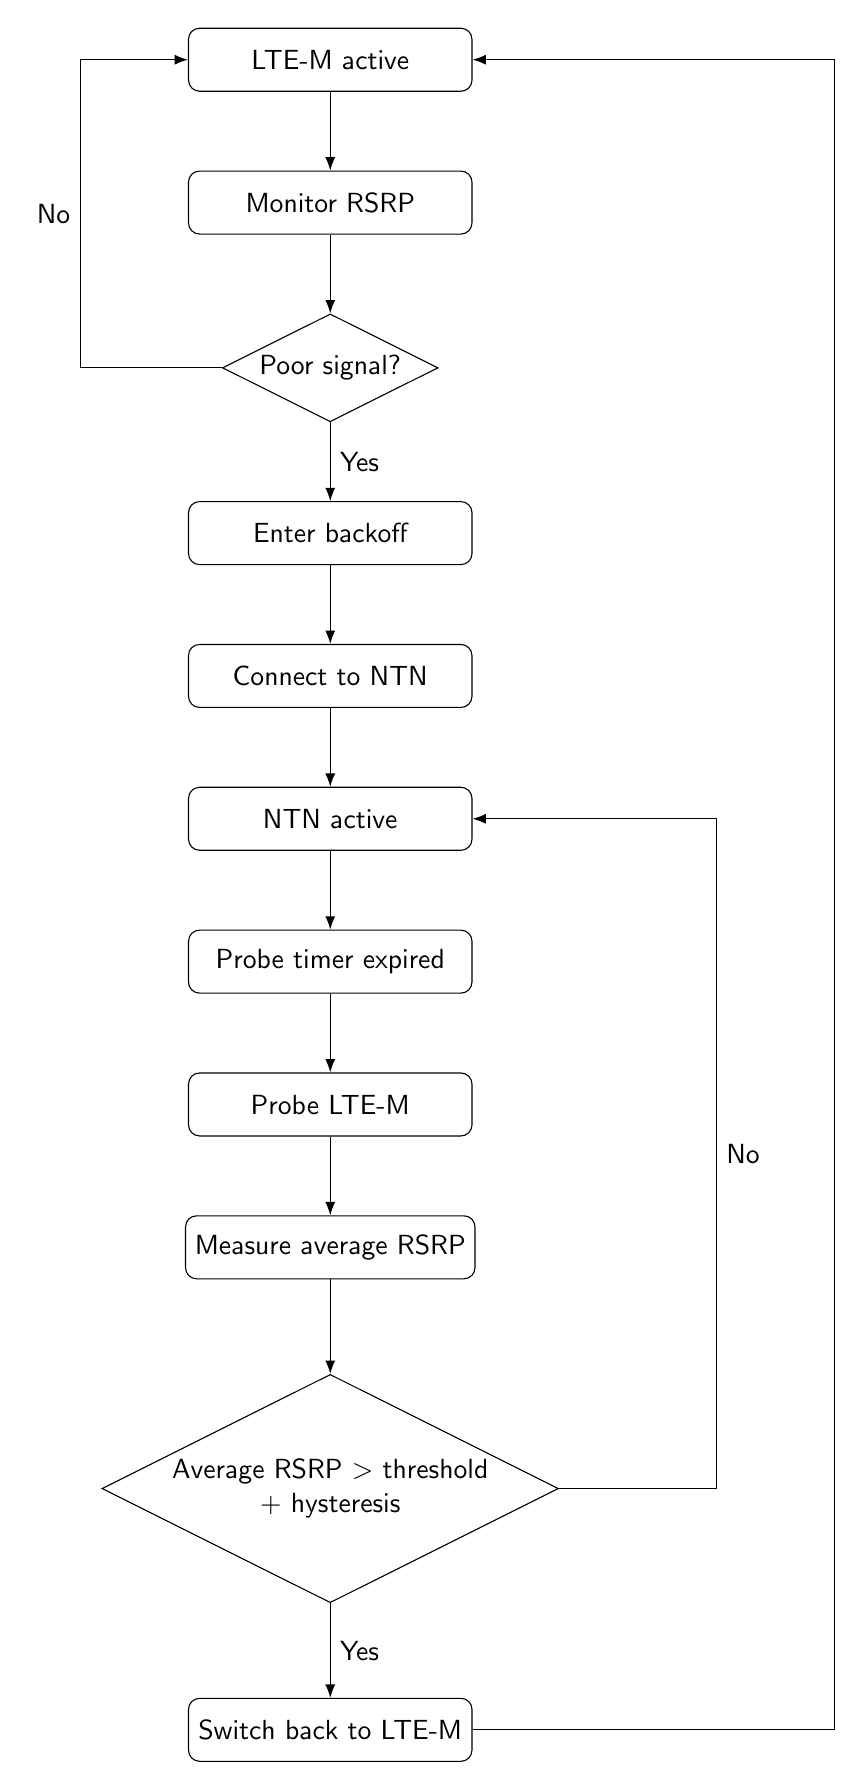
\begin{tikzpicture}[
    node distance=10mm and 16mm,
    % using shared TikZ defaults
]

\node[process] (A) {LTE-M active};
\node[process, below=of A] (B) {Monitor RSRP};
\node[decision, below=of B] (C) {Poor signal?};
\node[process, below=of C] (D) {Enter backoff};
\node[process, below=of D] (E) {Connect to NTN};
\node[process, below=of E] (F) {NTN active};
\node[process, below=of F] (G) {Probe timer expired};
\node[process, below=of G] (H) {Probe LTE-M};
\node[process, below=of H] (I) {Measure average RSRP};
\node[decision, below=12mm of I] (J) {
    Average RSRP $>$ threshold \\
    + hysteresis
};
\node[process, below=12mm of J] (K) {Switch back to LTE-M};

\draw[line] (A) -- (B);
\draw[line] (B) -- (C);
\draw[line] (C) -- node[right]{Yes} (D);
\draw[line] (D) -- (E);
\draw[line] (E) -- (F);
\draw[line] (F) -- (G);
\draw[line] (G) -- (H);
\draw[line] (H) -- (I);
\draw[line] (I) -- (J);
\draw[line] (J) -- node[right]{Yes} (K);
\draw[line] (K.east) -- ++(46mm,0) |- (A.east);

\draw[line] (C.west) -- ++(-18mm,0) |- node[pos=0.25,left]{No} (A.west);
\draw[line] (J.east) -- ++(20mm,0) |- node[pos=0.25,right]{No} (F.east);

\end{tikzpicture}
\end{document}
